\section {Overall design}

There are two distinct process types: persistent and non-persistent. The persistent processes will run for the entire uptime of the system whereas the lifetime of a non-persistent process is the duration of its given task. Figure \ref{fig:processhi} below shows the current system design.

\begin{figure}[h!]
	\centering
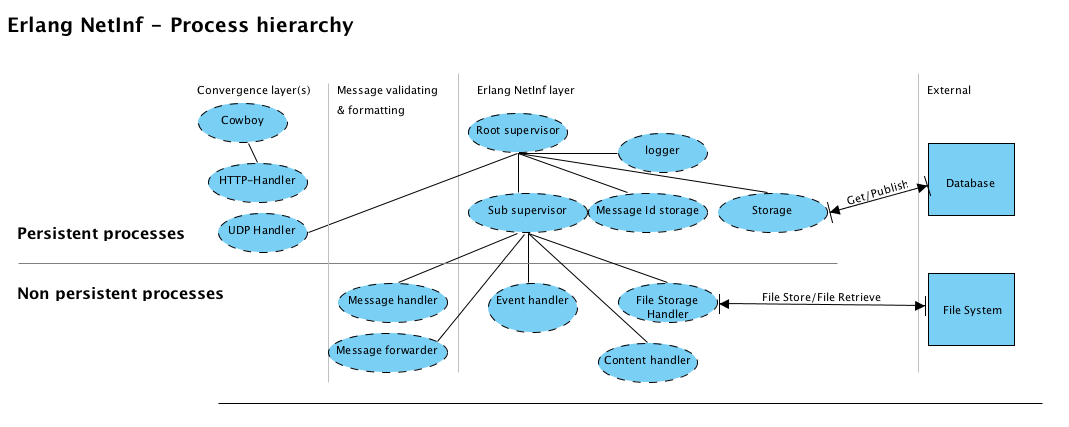
\includegraphics[scale=0.6]{./img/process_hierarchy.png}
\caption{Current system design}
\label{fig:processhi}
\end{figure}

\subsection{Architecture layers}

The system architecture is divided into three distinct layers a network layer (HTTP, UDP) convergence layer, an internal Erlang NetInf layer and a storage layer. Within these layers lies the modules(Erlang processes) which are responsible for specific functions such as sending/receiving convergence layer messages, sanitizing messages, forwarding, accessing databases/file systems and logging.

\subsection{NetInf Messaging}

According to the draft specification(see appendix D-draft) NetInf has three well defined messages which comprise of the core functionality of the system. The following sections describe the purpose and flow of each of these messages in addition to how the Erlang NetInf NRS handles them.

\subsubsection{Named Data Objects}
In addition to the messaging component, NetInf describes any piece of information as a Named Data Object(NDO). In the current state of networks, the same piece of information is considered to be location based and mutable with many copies of the same information lying around. The purpose of an NDO is to provide a convenient way for the protocol to be able to catalogue and preform operations such as storing, retrieving and finally searching for information while eliminating the need for location based information.

\subsubsection{Internal NetInf Messaging}

The Erlang NetInf NRS uses an internal record to represent a NetInf protocol message. For each request in the system, an instance of the following Erlang record is created and passed to various modules in order to have the specific operation preformed. Afterwards the NRS constructs a response message and sends it back to the requester. There are two records defined in the module nn\_proto, the first defines a request, primarily a Publish, Get, or Search messages from outside of the system(external clients and other NRS'). While the second record defines the NDO. The message record includes the NetInf record (if available). 

\label{NDO-message}
\begin{verbatim}
-record(message, 
	{
	  msgid = undefined :: term(),
	  time_to_live = undefined :: undefined | integer(),
	  octets = undefined :: undefined | binary(),
	  tokens = undefined :: undefined | [binary()],
	  method = undefined :: undefined | get | search | publish | error,
	  netinf = undefined :: undefined | proto() | [proto()] | term()
	}).
\end{verbatim}

The "netinf" field in the above record is dependent on the method and whether or not the message is a request or a response.

\begin{verbatim}
-record(netinf, {
	  % name of the ndo
	  name = undefined :: undefined | binary(),
	  % list of possible locations and or URI's
	  uri = [] ::[] | [binary()], % either empty list or a list of binary terms,
	  % list of extensions stored in json format
	  ext = {[]} :: {[]} | {[{binary(), any()}]}, 
	  % timestamp of the ndo in json format
	  time_stamp = undefined :: undefined | binary() 
	 }).
\end{verbatim}

\subsubsection{Publish}

NetInf describes a Publish message which consists of the following fields:

\begin{description}
\item[URI]  - Contains the hash of the NDO. It is unique to the piece of information that is going to be published into the system. It is also mandatory.
\item[msgid] - A mandatory field as well and it is a unique number(string). 
\item[loc1] - An optional field, this is a locator that can be used to access the information that will be shared.
\item[loc2] - Same as the above.
\item[ext] - An extension field, it is responsible for containing the metadata if any, in JSON format.
\item[rform] - The response format, The NetInf will format the response message using either HTML or JSON. JSON is the default if this field is not set. This is convergence layer specific.
\item[fullPut] - This field is set to determine if octets(binary data) is present with the publish message with either ''true'' or ''false''
\end{description}

\subsubsection{Publish Message Workflow}

A requester would like to share information. Using an external client the requester sends a NetInf Publish Request message with the mandatory fields set as described above through a supported convergence layer(HTTP for example). The Erlang NetInf NRS will then receive the message and create a 'message' record(see section: \ref{NDO-message}).

A convergence layer handler(CL handler) is spawned and receives the request.
Once a request is in the system, the CL handler that received it will pass the request onto the message handler(MH). The MH is independent of the CL however, the formatting library used by the MH will depend on the CL the request was received on.

At this point the original request will be validated and sanitized for use in the internal NRS system and a NDO will be created. If the request is malformed the MH will construct a response message immediately and pass the new message back, informing the requester of the specific reason the request was rejected and then the MH will die. 

In the case that the validation and sanitization succeeds the MH will have a newly sanitized and internal message representation of the original request(NDO). The request is now ready to be passed deeper into the system. The MH spawns an Event Handler(EH) and goes to sleep waiting for the message to complete the process. 

The Event Handler will then read the NDO and determine if a Content Handler(CH) will need to be spawned in order to store the binary data(octets). The CH is only spawned if the FullPut flag in the original request was present and set to 'true'. Finally the EH will pass the NDO to the Storage module and wait until the process is complete.

The Storage module will call the appropriate function for the database(through the functions defined in the Database Wrapper nn\_database). In this case the database will store the published NDO. If a NDO with the same name exists, the two NDO's are merged and the result is stored.

Once the NDO is stored in the database a message is sent back through the chain of waiting processes. This occurs until the Message formatter can create a response containing the NDO that was stored and any CL specific response codes. Note that any process' that were temporarily spawned will kill themselves after the job is complete. Figure XX shows the flow of communication for Publish requests.  


\subsubsection{Get}

NetInf describes a Get message which consists of the following fields:

\begin{description}
\item[URI] - Contains the unique hash of the NDO as well as the hash algorithm. The user requests the specific data object using this hash.
\item[msgid]- A mandatory and unique number for each message in the system.
\item[loc1] - Same as above
\item[loc2] - Same as above
\item[ext]  - A field reserved for future extensions.
\end{description}

\subsubsection{Get Message Workflow}

A requester would like to retrieve information, using an external client the requester sends a NetInf Get request(assuming they know the name of the NDO they are looking for) in the format described above. The process is similar to the publish, until the NDO is passed to the event handler. The event handler will call the database to lookup the NDO using the URI field. If found the NDO will be returnd back through the system to the Message Formatter in order to construct the appropriate response message. However, if the NDO is not found a Message Forwarder will be spawned and the NDO request is broadcasted out on the UDP CL. If there are other Erlang NetInf NRS' on the network a UDP response packet will be sent and the original NRS which forwarded the request will eventually respond to the requester with the NDO or timeout. Figure XX shows the flow of communication for Get requests.

\subsubsection{Search}

NetInf describes a Search message which consists of the following fields:

\begin{description}
\item[msgid] - Mandatory and a unique number.
\item[tokens] - Space delimited text. This is the text that the user will search for within the system
\item[rform] - Optional and will default to Json if not specified, however this is convergence layer specific.
\item[ext] - A optional field reserved for future extensions.
\end{description}

\subsubsection{Search Message Workflow}

A requester would like to retrieve information but they does not know the name of the NDO. A NetInf search request can be sent to the Erlang NetInf NRS to retrieve a list of NDO names and the metadata which match a particular criteria(search tokens). The process is similar to both the Get and the Publish however the event handler calls the appropriate search function in the attached database. If no match is found the request is automatically forwarded on the UDP CL where the same procedure takes place. If a match is found, a response is created  and sent back to the original CL handler. Figure XX shows the flow of communication for  Search requests.
